\documentclass{beamer}

\mode<presentation> {
	

	\usetheme{Boadilla}
	
	
	\usecolortheme{seagull}  %plain
	
}
\usepackage{hyperref}
\usepackage{graphicx} % Allows including images
\usepackage{booktabs} % Allows the use of \toprule, \midrule and \bottomrule in tables

%----------------------------------------------------------------------------------------
%	TITLE PAGE
%----------------------------------------------------------------------------------------

\title[Django Workshop]{Django Workshop Introduction} % The short title appears at the bottom of every slide, the full title is only on the title page

\author{Advanced Programming} % Your name
\institute[AUT] % Your institution as it will appear on the bottom of every slide, may be shorthand to save space
{
	Amirkabir University of Technology\\ % Your institution for the title page
	\medskip
	\textit{} % Your email address
}
\date{Winter 2019} % Date, can be changed to a custom date

\begin{document}
	
	\begin{frame}
		\titlepage % Print the title page as the first slide
	\end{frame}

	\begin{frame}
	\frametitle{Overview} % Table of contents slide, comment this block out to remove it
	\tableofcontents % Throughout your presentation, if you choose to use \section{} and \subsection{} commands, these will automatically be printed on this slide as an overview of your presentation
	\end{frame}

%	PRESENTATION SLIDES

\section{What is Django} 
\begin{frame}
\frametitle{What is Django}
	\begin{enumerate}
	\item Django is a free and open-source web framework written in python.
	\item It supports MVC architectural pattern. 
	\item Django Software Foundation is an independent 
	organization who is responsible for the maintenance of django framework.
	\end{enumerate}
\end{frame}

\begin{frame}
	\begin{figure}
		
\includegraphics[width=\linewidth]{Pics/PyDjango.jpg}
	\end{figure}
\end{frame}
\subsection{Free and Open-Source}
\begin{frame}
\frametitle{Free and Open-Source}
\begin{itemize}
	\item It was initially released by Adrian Holovaty and Simon Willson on 21 July 2005.
	\item Repository: \href{github.com/django/django}{github.com/django/django}
	\item Website: \href{www.djangoproject.com}{www.djangoproject.com}
\end{itemize}
\end{frame}


\subsection{Web Framework}
\begin{frame}
	\frametitle{Why Using a Framework?}
	\begin{block}{Web Framework}
		A web framework is a group of software structures, designed to support development of web application. We as developers, use frameworks to be provided with a unique and standard approach.
	\end{block}

	\begin{itemize}
		\item We can map requested URL from user to the code we have written.
		\item We can inject calculated values and information from database that leads to dynamic HTML files.
	\end{itemize}
\end{frame}


\subsection{Python}
\begin{frame}
\frametitle{Why Coding in Python?}
\begin{itemize}
	\item There is a growing community of developers waiting for you.
	\item Less lines of code means less chance of facing bugs and easier maintenance over time.
\end{itemize}
\begin{figure}
	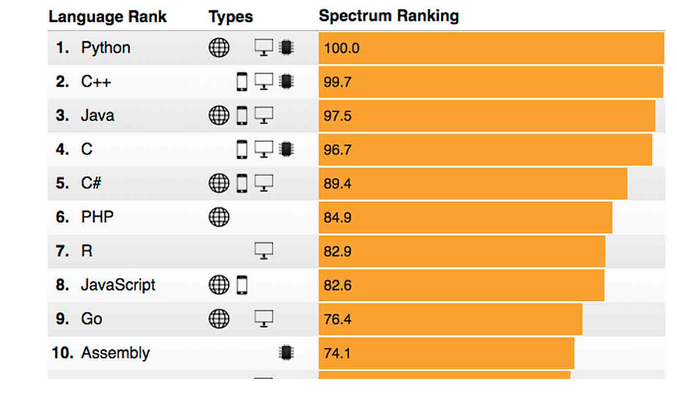
\includegraphics[width=0.7\linewidth]{Pics/python_ranking.png}
	\caption{IEEE spectrum latest ranking}
\end{figure}
\end{frame}

\subsection{MVC}
\begin{frame}
\frametitle{What is MVC or MVT?}
MVC architectural pattern enables us to make Data layer, Presentation layer and Business Logic layer isolated. As a result our project will be easier to maintain and understand. It loosens the coupling between each layer of project and improves modularity and cohesion of code.
\begin{block}

\begin{itemize}
	\item "M" stands for Model. It is our gateway to database and models.py is responsible for this purpose.
	\item "V" stands for View. It is the representation of the application to the end user and Templates are responsible for this purpose.
	\item "C" stands for Control. It is the implementation of the underlying logic behind our project and views.py plays this role in a django project.
\end{itemize}
\end{block}
	considering the beginning of names "models.py", "views.py" and "templates", makes it possible for us to use MVT and MVC interchangeably.
\end{frame}

\begin{frame}
\frametitle{MVT in Practice}
This is how a Django web application works:
\begin{figure}
	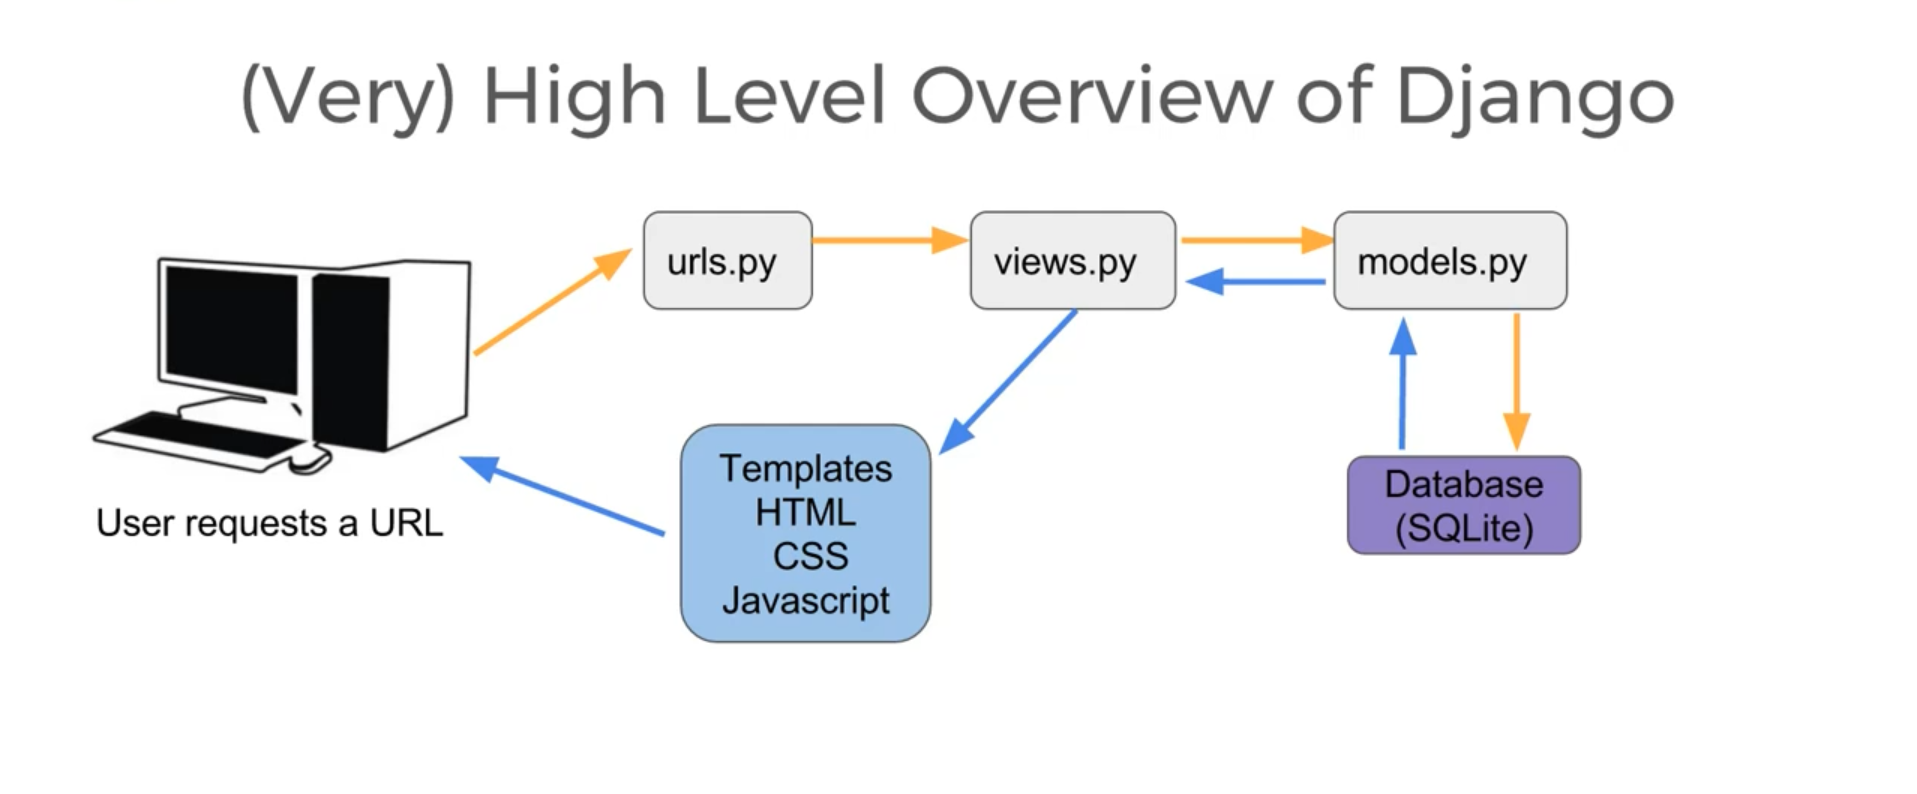
\includegraphics[width=\linewidth]{Pics/High_level.png}
\end{figure}
\end{frame}

\subsection{Maintenance}
\begin{frame}
	\frametitle{Maintenance}
	\begin{itemize}
		\item It is highly maintained by Django Software Foundation.
		\item The latest released version is 2.1.5 that has been committed in January 2019.
		\item There will be new features, bug-fixes and security improvements every now and then.
		\item there are dozens of free books, online tutorials and a strong documentation provided.
	\end{itemize}
\end{frame}

\section{Why Using Django?}

\subsection{Fast}
\begin{frame}
\frametitle{Why Using Django? (1)}
	
	\begin{itemize}
		\item Low coupling, rapid development, and the principle of don't repeat yourself.
		\item Reusability of modules (apps) and pluggability of components (tools)
	\end{itemize}

	\begin{figure}
		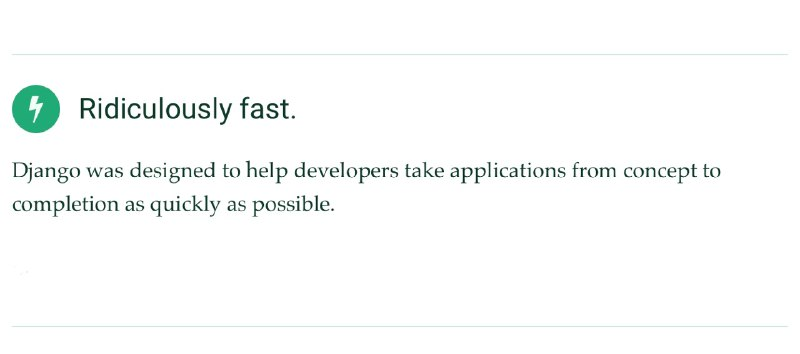
\includegraphics[width=0.8\linewidth]{Pics/Django/index.jpeg}
	\end{figure}
\end{frame}

\subsection{Equipped}
\begin{frame}
\frametitle{Why Using Django? (2)}
\begin{itemize}
	\item Django Admin helps us authenticate users and other administrative work easily.
	\item Django officially supports four database backends: PostgreSQL, MySQL, SQLite, and Oracle.
	\item There are many servers who offer free deployment facilities for django projects.
\end{itemize}
\begin{figure}
	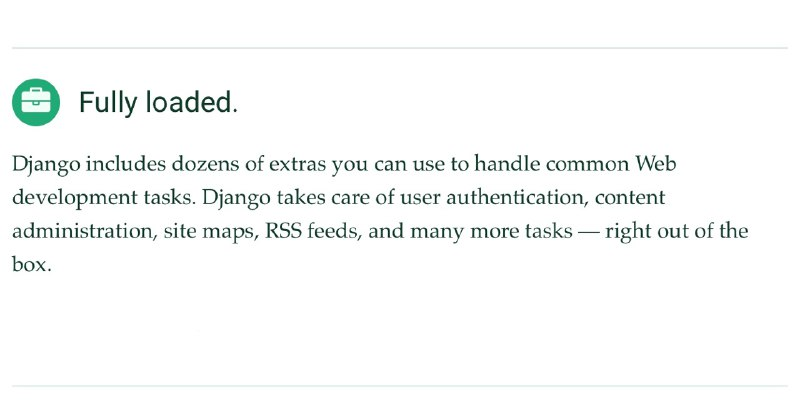
\includegraphics[width=0.8\linewidth]{Pics/Django/index2.jpeg}
\end{figure}
\end{frame}

\subsection{Secure}
\begin{frame}
\frametitle{Why Using Django? (3)}
\begin{figure}
	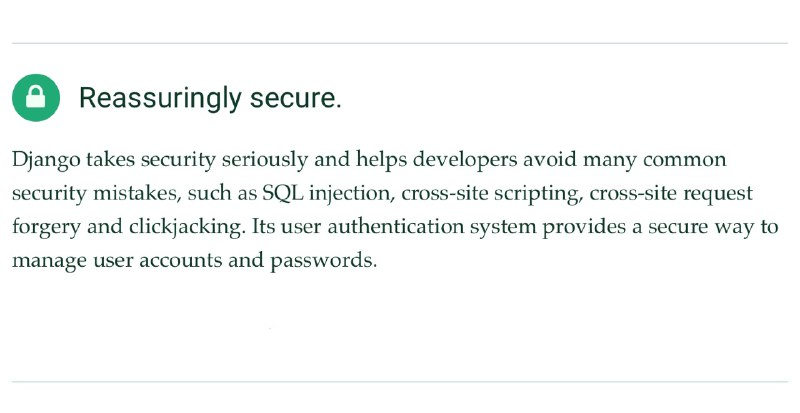
\includegraphics[width=0.8\linewidth]{Pics/Django/index3.jpeg}
\end{figure}
\end{frame}

\subsection{Scalable}
\begin{frame}
\frametitle{Why Using Django? (4)}
\begin{figure}
	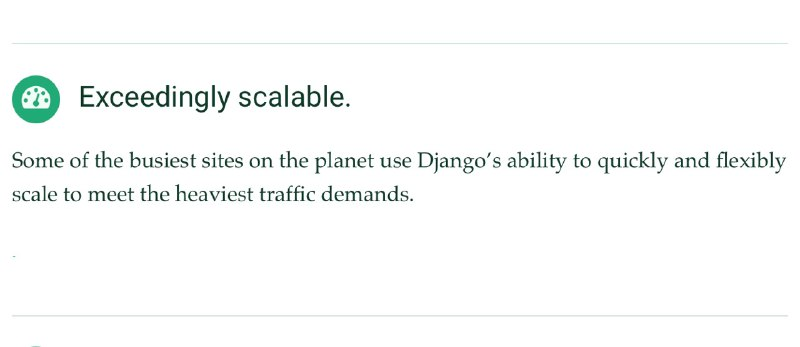
\includegraphics[width=0.8\linewidth]{Pics/Django/index4.jpeg}
\end{figure}
\end{frame}

\subsection{Versatile}
\begin{frame}
\frametitle{Why Using Django? (5)}
\begin{figure}
	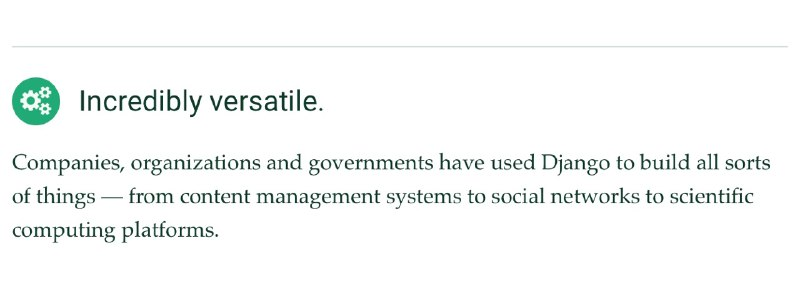
\includegraphics[width=0.8\linewidth]{Pics/Django/index5.jpeg}
\end{figure}
\end{frame}

\section{Where to Use Django}
\begin{frame}
	\frametitle{Django in Real World}
	Here are some of the most well-known websites using Django most of which are social networks:
	
	\begin{itemize}
		\item Public Broadcasting Service (PBS)
		\item Instagram
		\item Spotify
		\item YouTube
		\item Dropbox
		\item Mozilla
		\item The Washington Times
		\item Disqus
		\item Bitbucket
		\item Nextdoor
		\item Pinterest
		\item .....
	\end{itemize}
\end{frame}

\begin{frame}
	\frametitle{What Will We Do With Django?}
	In following sessions after getting familiar with basics of python and django, we will get into making a simple blog project. It has two major phases and we will add new features to it step by step.
	Finally, you can develop your own blog website for sharing your posts, curriculum vitae etc.
\end{frame}

\begin{frame}
\frametitle{References}
	\href{https://en.wikipedia.org/wiki/Django_(web_framework)}{https://en.wikipedia.org/wiki/Django-(web-framework)}
	\href{https://www.djangoproject.com/}{https://www.djangoproject.com/}
\end{frame}

\begin{frame}
\Huge{\centerline{The End}}
\end{frame}

\end{document} 